% !TeX root =../../main.tex

\chapter{The FOT Fuzzing Framework} \label{ch:fot}


\section{Introduction and Motivation}


In spite of the popularity and effectiveness of applying greybox fuzzing techniques in detecting vulnerabilities(c.f. Sec~\ref{sec:intro-gbf}), there does not exist a general greybox fuzzing framework to reuse, integrate and evaluate fuzzing extensions as well as try new techniques.
For example, {\AFL}'s core fuzzing logic, around 8000 lines of code, all resides in one single file, with more than 100 global variables. Therefore, the integration of one new feature often involves modifications in multiple places; this changes are usually erroneous since a minor mistake may cause whole logic wrong.
In reality, {\AFL} is highly coupled as it is designed with limited options for configurations~\cite{afl}.
Further, most of the existing fuzzers are extensible to integrate with new features.
Hence, a fuzzing framework is preferred to allow for both easy \emph{configuration} and \emph{extension}.


In this sense, we propose our fuzzing framework, \emph{Fuzzing Orchestration Toolkit} ({\FOT}), which has the following three properties.

\begin{enumerate}[(1)]
\item  \textbf{Versatility.}
{\FOT} provides a fuzzing toolkit, including static analysis enhanced fuzzing preprocessors, collaborative fuzzing core, as well as a set of toolchains for additional analysis purpose.
\item \textbf{Configurability.}
{\FOT} has builtin support for multiple configuration options, which makes it easy to tweak fuzzing parameters in order to improve the overall fuzzing effectiveness.
\item \textbf{Extensibility.}
{\FOT} consists of the library for general-purpose fuzzing utilities, as well as the miscellaneous tools on top of it, which makes it possible for developers to customize their own fuzzers with modest efforts.
\end{enumerate}


\section{Architecture}\label{sec:details}

\begin{figure}[ht]
	\centering
	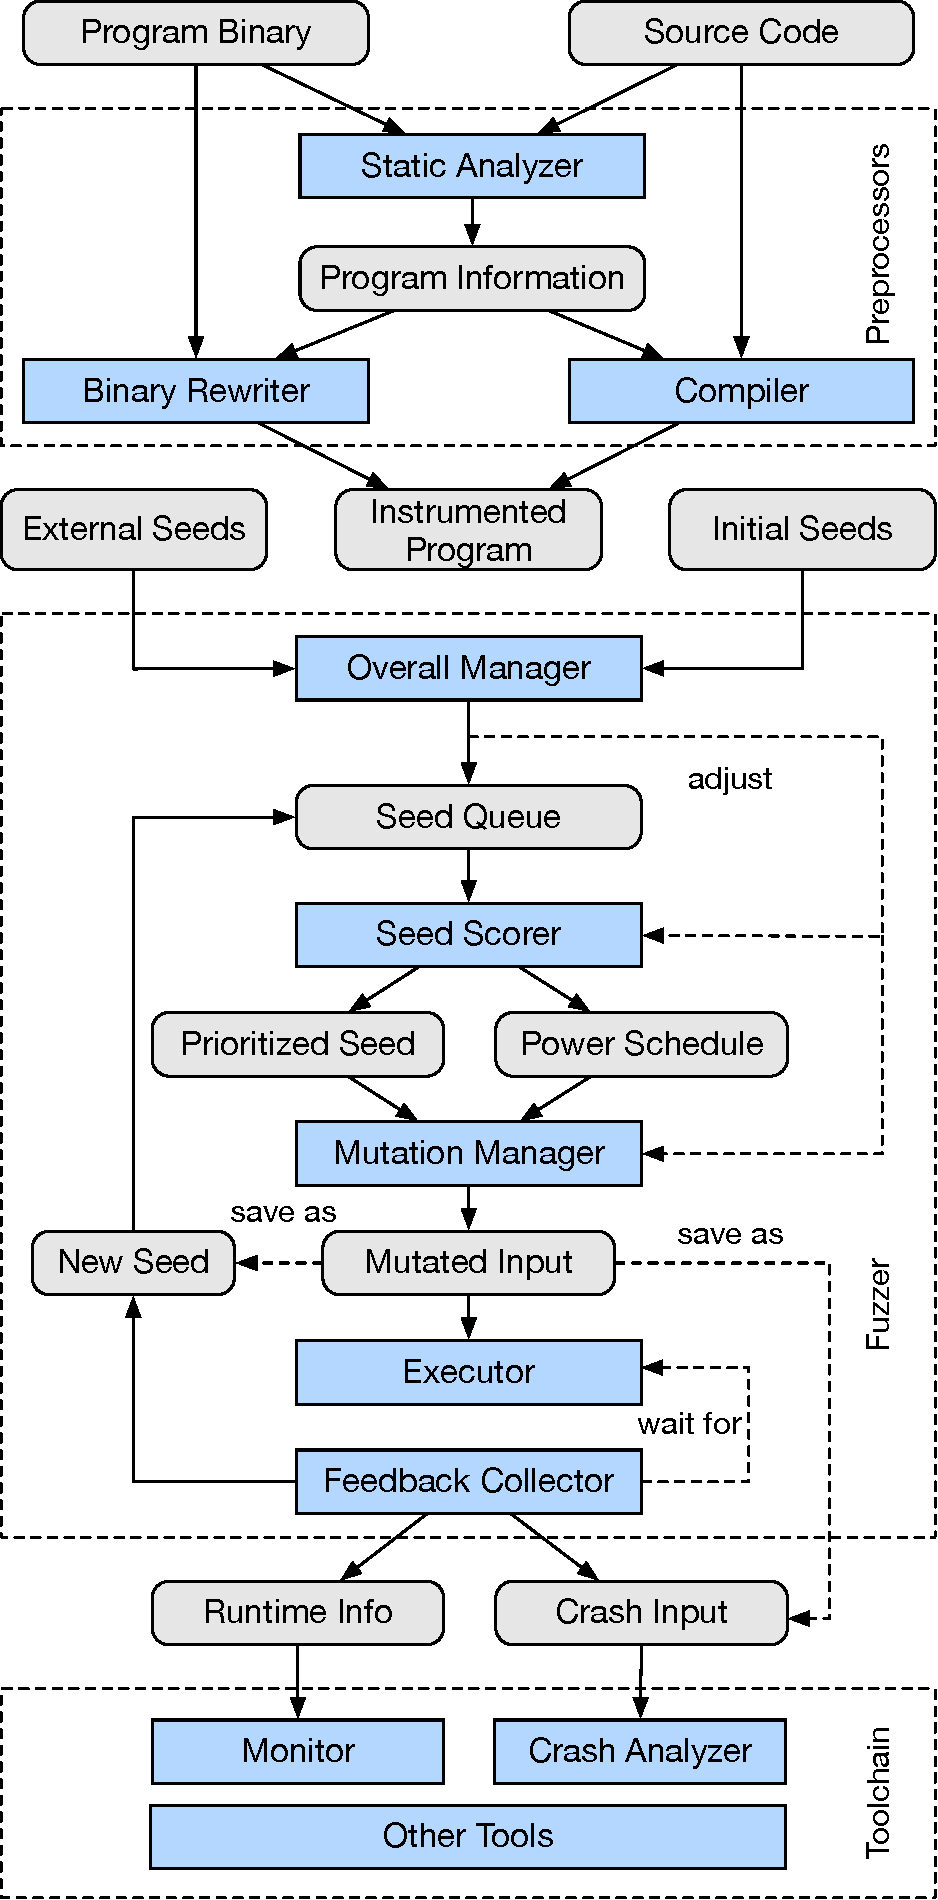
\includegraphics[width=0.5\textwidth]{res/fot/FOT_overview}
	\caption{The architecture of the {\FOT} fuzzing framework}
	\label{fig:fot_workflow}
\end{figure}

This section describes the key components of {\FOT}.
Figure~\ref{fig:fot_workflow} depicts the overall architecture of {\FOT}.
It has three parts (labeled in pink): the \emph{preprocessor}, the \emph{fuzzer}, and the \emph{complementary toolchains}.
The components are labeled in \emph{blue} while the inputs and inputs/outputs are in \emph{grey}.


\subsection{Preprocessor}
This part consists of multiple tools to collect statically calculated metrics which will be encoded as instrumentation stubs inside the target programs.


\subsubsection{Static Analyzer}\label{sec:static_analysis}
This includes several analyzers to extract interesting semantics from the target program, such as control flow graph generation, data flow analysis results, as well as the metric utility to fit them for instrumentation.
It is \textit{configurable} to generate different levels of static information. It is \textit{extensible} as developers are allowed to add new types of static analysis as long as the generated result follows the specified format.


\subsubsection{Instrumentor}
\emph{Binary rewriter} and \emph{source transformer} instrument static results generated by the static analyzer into the target program for the fuzzer to collect feedback during runtime execution.
{\FOT} supports LLVM based transformation when the source code is available, and Dyninst~\cite{dyninst} rewriting when only the binary is provided.
It is \textit{configurable} since it allows instrumentation either on source code or binary.
It is \textit{extensible} since developers can use other instrumentors (e.g., Intel PIN~\cite{pin}), as long as the instrumented code can embed the static information and provide sufficient feedback during fuzzing.

\subsection{Fuzzer}
This part deals with the actual fuzzing. 
Basically, the core of fuzzing is a loop that continuously picks seeds from a seed queue, applies mutations on the seeds, executes the target program against seed variants, and collects statistics for subsequent iterations.

\subsubsection{Conductor}
{\FOT} a \emph{conductor} to schedule workloads of different workers. This specifically allows for parallel fuzzing in a multithreading mode by collaborating different fuzzing instances. In addition, a monitoring worker can also be woke up regularly to retrieve seed inputs from external tools, including symbolic executors (e.g., KLEE~\cite{klee}), random seed generators (e.g., Radamsa~\cite{radamsa}), by monitoring a specific seed directory.
It is \textit{configurable} since end-users are allowed to choose different fuzzing modes.
It is \textit{extensible} since it can interoperate with other external tools.


\subsubsection{Seed Scorer}
The seed scorer is in charge of selecting a seed from the queue for mutation (seed selection) and determining how many new seeds are to be generated from the selected seed (power scheduling).
It is \textit{configurable} since end-users can choose builtin scoring strategies to evaluate seeds.
It is \textit{extensible} since developers can implement their own strategies with the provided interfaces.


\subsubsection{Mutation Manager}
The mutation manager schedules different kinds of mutators, which includes bitwise flips, bytewise flips, arithmetic operations on bytes, byte chunk addition, modification or deletion, crossover between two seeds, etc.
It is \textit{configurable} as {\FOT} has various mutators (and their combinations) for end-users to choose from.
It is \textit{extensible} as developers can implement their own mutators with the provided interfaces.

\subsubsection{Program Executor}
The program executor drives the execution of the target program.
It is \textit{configurable} since the default executor in {\FOT} allows end-users to choose whether or not to use forkserver~\cite{afl} during fuzzing.
It is \textit{extensible} since developers can extend the program executor for various scenarios.
For example, they may add a secondary executor to execute another program for differential testing.

\subsubsection{Feedback Collector}
The feedback collector collects the runtime feedback based on the instrumented information (e.g., path coverage) as well as the program's execution status.
It is \textit{configurable} as end-users are allowed to select from the builtin feedback options.
For now, the feedback can be at basicblock level (same as {\AFL}) or function level (specific to \FOT).
It is \textit{extensible} as end-users can specify their customized types of feedback for collection.

\subsection{Complementary Toolchains}
{\FOT} contains various complementary tools which help to make the framework \textit{versatile}.
For instance, we implemented a web-based frontend user interface to observe the overall results, which provides intuitive and fruitful information for manual monitoring.
We also have a crash analyzer to analyze the detected crashes and automatically generate reports.
This greatly reduces the manual efforts of crash triaging.
Many other tools are also being added to complement the fuzzer.


%\begin{figure}[t]
%	\centering
%	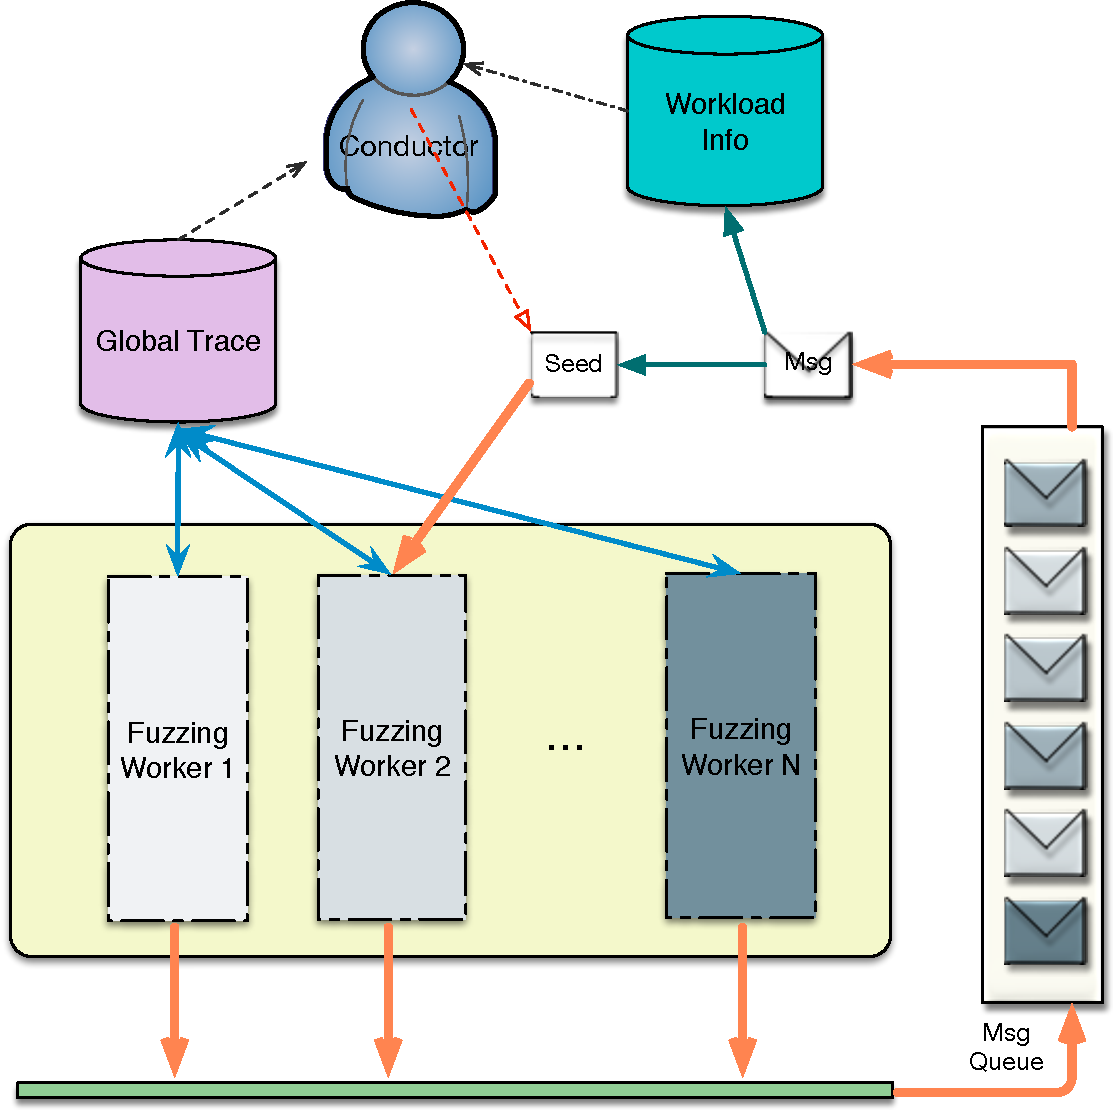
\includegraphics[width=0.56\columnwidth]{res/fot/mt_workflow}
%	\caption{Coordination among Different Fuzzing Instances}
%	\label{fig:mt_workflow}
%\end{figure}


%\subsection{Trace Update and Synchronization}\label{sec:trace_sync}
%One of {\FOT}'s key features is the builtin coordination among different fuzzing instances (Figure~\ref{fig:mt_workflow}). One important issue is the trace synchronization between fuzzing instances. For instrumentation, we made a slight change to the conventional instrumentation runtime to enable the target binaries to distinguish different shared memory arenas and the file descriptors used for ``forkserver'' allocated by different fuzzing instances. Each fuzzing instance allocates the shared memory and the instrumented binary writes to specific multiple 8-byte areas when the corresponding ``execution edges'' have been reached. By auditing the byte fingerprints, the fuzzer knows about the edges and their approximate hit counts within this run. This information sits between between ``branch coverage'' and ``path coverage''. By comparing the shared memory fingerprint with the local trace information (checking whether the active shared memory byte has been marked ``traced'' locally), the fuzzer gets the knowledge whether current running seed increases the coverage. Updating of the local trace is majorly a ``bitwise and'' where each byte of the local trace is initialized with all ones (i.e., 255).
%
%The local trace is synchronized with the global trace state. There stands a tradeoff: if we use directly the global trace state, the synchronization will be too frequent and eventually decreases performance with the increase of more fuzzing instances; if the fuzzers are only aware of the local trace, it is no better than {\AFL}'s na\"ive approach that runs all instances separately. We thus choose to only apply the synchronization during the mutation of each seed in the queue, when customizable conditions are triggered.
%% (usually the conditions are about the executions and time since last synchronization).
%
%The actual synchronization of the trace information applies ``bitwise and'' on normal running traces from local trace information to global state, and an instant copy in the other direction. This is far more efficient than {\AFL}'s synchronization by 1) importing seeds from other directories and 2) running all the seeds indistinguishably. Note that {\FOT}'s synchronization does not lose precisions compared to {\AFL}'s, where both ``bitwise and'' operations erase the exact hit count information.


%  \subsection{Mutation Strategy Adaption}\label{sec:mutation_ops}
% The selection of mutation operators on one seed in the queue is determined by:
% \begin{enumerate}[1.]
% 	\item The whitelist mutation operators used for the targeted binaries. Some mutation operators are only effective on certain programs, but is almost a waste of time for the other programs (for example, bitflip operations are quite expensive and rarely useful for text-based parser programs running against large files). This can be specified by the experienced {\FOT} end-users.
% 	\item The one-time mutation operators for \emph{this turn}. This is automatically determined by the fuzzer according to statistics generated from the previous mutations and runs. It is calculated in an adaptive way and may finally help to determine the ``convergence'' of the seeds.
% \end{enumerate}
%
%%On the other hand, {\AFL} has rather limited configurations for what mutation operators can be used and frequently runs blindly on the mutations that do not fit well~\cite{junjie:2017sp:skyfire,mopt-fuzz}.
%
%
%\subsection{Refinement on Variable Behaviors}\label{sec:entry_var_behavior}
%
%Some programs have variable behaviors for the same seed, due to randomness, multi-threading, etc. {\AFL} handles this issue by running all the newly found interesting seed multiple times (known as \emph{calibration}); whenever it finds that the shared memory information (the active bytes and their hit count) differs from the first run, it will give more chances to the running seed entry, and then keeps track of the variable behavior rate. The problem is that it does not utilize the information further since variable behaviors may cause certain runs to exit normally at some time, however crash at other time, which is more serious. We separately track those seeds and give even more chances for them. Alternatively, we provide an intrinsic strategy to prioritize these cases and let those seeds to be more likely to run next time. On the other hand, {\AFL}'s tracing information for the variable behavior cases are imprecise since it only traces the last calibration shared memory; we refine this by (selective) ``bitwise or'' operations to the shared memory for subsequent procedures on the current seed.
%
%
% \subsection{Trimming on Duplicated Cases}
%Due to the existence of the potential lag of the trace synchronization, there still exist some seeds that run with the same running trace. In other cases, certain seeds might not be in its ``simplest'' form: by removing some bytes, the seed can still result in the same running trace. {\FOT}'s approach in handling this is to trim the calibrated seeds immediately before being parceled as the message and sent to the message queue buffer managed by the conductor. And the conductor maintains a checksum set of all the generated seed files. Therefore when the newly generated seed has the same checksum as one of the existing ones, this seed will be discarded.
%
%We also provide an external minimizer to prune all the serialized seeds (including normal runs, timeout runs, or crashes); it is more aggressive than the embedded procedure in the fuzzer and aims to provide a minimized version of all the interesting seeds.
 

\subsection{Implementation}\label{sec:fot-impl}

The {\FOT} project started from June, 2017 and has been actively developed by two researchers. It is implemented with 16000 lines of Rust for core fuzzing modules, together with 4500 lines of C/C++ for the preprocessor, 4200 lines of Java for structure-aware mutation, and 2400 lines of Python for complementary toolchain.
  

\section{Relations with Other Fuzzing Tools}


%In this section, we first compare FOT with other fuzzing frameworks, and then discuss its relationship to current fuzzing extensions.



Table~\ref{tbl:cmp_fuzz} compares {\FOT} with existing fuzzing frameworks with respect to 10 fuzzing features. As we can see, the existing fuzzing frameworks, AFL, libFuzzer, and honggfuzz, lack \FOT's features in various aspects. {\FOT} stands out in that it provides multiple configurations for advanced end-users; it is also highly modularized, suitable to be extended with other fuzzing techniques.
%Moreover, {\FOT} partially supports structure-aware mutations and interoperability with other external tools such as symbolic executors (by monitoring and scheduling newly incoming seed directory).

Most current fuzzing extensions can be easily integrated into {\FOT} owing to its design. In reality, they can be applied with some extensions to the different components in Figure~\ref{fig:fot_workflow} and can be used together with the configuration interface. 

\begin{enumerate}[1)]
	\item \dFOT is implemented by applying target location specific static analysis, as well as optimizations on seed selection, power scheduling, mutations.
	\item \mtfuzz is implemented by applying thread-aware static analysis and special instrumentations, as well as the optimizations on seed selection, power scheduling strategies, program executor, feedback collector, etc.
	\item AFLFast~\cite{Bohme:2016:CGF} can be implemented by applying a Markov Chain model based seed \emph{power scheduling} in the fuzzer. 
	\item AFLGo~\cite{Bohme:2017:DGF} can be implemented by a combination of \emph{static analyzer}, \emph{instrumentation} and \emph{power scheduling}.
	\item CollAFL~\cite{CollAFL} can be implemented by using a collision-resistant algorithm to increase the uniqueness of the path trace labeling during \emph{instrumentation}.
	\item Skyfire~\cite{junjie:2017sp:skyfire}, Radamsa~\cite{radamsa}, Csmith~\cite{csmith} can be used to generate \emph{external seeds} which will be \emph{imported}, or integrated as structure-aware mutators conducted by \emph{mutation manager}. Symbolic executors such as KLEE~\cite{klee} can be integrated in the Driller's~\cite{driller} style with the help of \emph{conductor}.
\end{enumerate}

\begin{table}[t]
\centering
	\small
	\caption{Comparisons between fuzzing frameworks (\Circle: not supported, \LEFTcircle: partially supported, \CIRCLE: fully supported)}
	\label{tbl:cmp_fuzz}
	\begin{tabular}{|l|c|c|c|c|}
		\hline
		\diagbox{\textbf{Features}}{\textbf{Framework}} & \textbf{AFL} & \textbf{libFuzzer} & \textbf{honggfuzz} & \textbf{FOT} \\ \hline\hline
		Binary-Fuzzing Support & \CIRCLE & \Circle & \CIRCLE & \CIRCLE \\ \hline
		Multi-threading Mode & \Circle & \CIRCLE  & \CIRCLE  & \CIRCLE  \\ \hline
		In-memory Fuzzing &\CIRCLE  & \CIRCLE &\CIRCLE  & \CIRCLE \\ \hline
		Advanced Configuration & \Circle  & \LEFTcircle  & \Circle  & \CIRCLE  \\ \hline
		Modularized Functionality & \Circle & \LEFTcircle & \Circle & \CIRCLE \\ \hline
		Structure-aware Mutation & \Circle  &\Circle & \Circle  & \LEFTcircle \\ \hline
		Interoperability & \Circle & \Circle & \Circle & \LEFTcircle \\
		\hline
		Toolchain Support &  \CIRCLE & \Circle  & \Circle  & \CIRCLE \\ \hline
		Precise Crash Analysis & \Circle  & \Circle  & \CIRCLE  & \CIRCLE  \\ \hline
		Runtime Visualization & \LEFTcircle & \Circle & \Circle & \CIRCLE \\ \hline
	\end{tabular}
\end{table}


\subsection{Newly Detected Vulnerabilities}

{\FOT} has been used to fuzz more than 100 widely used open source projects and it has detected more than 200 vulnerabilities, among these 51 CVE IDs have been assigned. The detailed information is available at Appendix~\ref{app:bugs}. Notably, \FOT has detected multiple vulnerabilities with \emph{high} or \emph{critical} severity. For example, CVE-2019-9169~\cite{CVE-2019-9169} stresses a vulnerability in the GNU C Library (a.k.a. glibc or libc6 on Linux distributions) through 2.29, where the function \func{proceed\_next\_node} inside POSIX regular expression (regex) component has a heap-based buffer-over-read via an attempted case-insensitive regex match. Thanks to the interoperability with the regex generators, FOT is able to generate more meaningful seeds that cover more corner cases of the regex components. According to CVSS v3.0~\cite{cvss3}, it is scored 9.8 out of 10.0 (critical severity); according to CVSS v2.0~\cite{cvss2}, it has a score of 7.5 (high severity). As a comparison, the notorious HeartBleed (CVE-2014-0160) is scored 5.0 medium severity according to CVSS v2.0 (no CVSS v3.0 for it). Many of other vulnerabilities discovered by \FOT also have high severity, e.g, CVE-2018-15822, CVE-2018-14394, CVE-2018-14395 in FFmpeg, CVE-2018-19837, CVE-2018-19838, CVE-2018-19839, CVE-2018-20821, CVE-2018-20822 in libsass, CVE-2018-14560, CVE-2018-14561, CVE-2019-11470, CVE-2019-11472 in ImageMagick, and CVE-2019-11473, CVE-2019-11474 in GraphicsMagick. We envision that with more integrated techniques, \FOT will have the capabilities to detect more vulnerabilities that are hard to be revealled by existing fuzzers.
